\documentclass[12pt,preprint]{aastex}
%\documentclass[12pt,preprint]{emulateapj}
\usepackage{amssymb,amsmath}
\usepackage{color,hyperref}
\newcounter{address}
\setcounter{address}{1}
\newcounter{tableone}
\newcounter{tabletwo}
% hypertex insanity
\definecolor{linkcolor}{rgb}{0,0,0.25}
\hypersetup{
  colorlinks=true,        % false: boxed links; true: colored links
  linkcolor=linkcolor,    % color of internal links
  citecolor=linkcolor,    % color of links to bibliography
  filecolor=linkcolor,    % color of file links
  urlcolor=linkcolor      % color of external links
}
\setlength{\emergencystretch}{2em}%No overflowing references
\newcommand{\eqnnumber}{equation}
\newcommand{\eg}{e.g.}
\newcommand{\ie}{i.e.}
\newcommand{\Ie}{I.e.}
\newcommand{\etal}{et~al.}
\newcommand{\Hipparcos}{\textsl{Hipparcos}}
\newcommand{\Gaia}{\textit{Gaia}}
\newcommand{\Tycho}{Tycho}
\newcommand{\gcs}{\textit{Geneva-Copenhagen Survey}}
\newcommand{\gcsabb}{GCS}
\newcommand{\normal}{{\cal N}}
\newcommand{\wishart}{{\cal W}}
\newcommand{\dirichlet}{{\cal D}}
\renewcommand{\vec}[1]{\mathbf{#1}} % boldface for vectors
\newcommand{\inv}{^{-1}}
\newcommand{\rr}{\vec{r}}
\newcommand{\bb}{\vec{b}}
\newcommand{\cc}{\vec{c}}
\newcommand{\ee}{\vec{\hat{e}}}
\newcommand{\mm}{\vec{m}}
\newcommand{\vv}{\vec{v}}
\newcommand{\xx}{\vec{x}}
\newcommand{\zz}{\vec{z}}
\newcommand{\ww}{\vec{w}}
\newcommand{\bij}{\bb_{ij}}
\newcommand{\bbij}{\bij}
\newcommand{\cci}{\cc_i}
\newcommand{\eex}{\vec{\hat{x}}}
\newcommand{\eey}{\vec{\hat{y}}}
\newcommand{\eez}{\vec{\hat{z}}}
\newcommand{\eer}{\vec{\hat{r}}}
\newcommand{\mmj}{\mm_j}
\newcommand{\mmk}{\mm_k}
\newcommand{\mmrj}{m_{r,j}}
\newcommand{\vvi}{\vv_i}
\newcommand{\vvj}{\vv_j}
\newcommand{\wwi}{\ww_i}
\newcommand{\wwj}{\ww_j}
\newcommand{\wwk}{\ww_k}
\newcommand{\ten}[1]{\mathbf{#1}} % boldface for tensors
\newcommand{\BB}{\ten{B}}
\newcommand{\CC}{\ten{C}}
\newcommand{\UU}{\ten{U}}
\newcommand{\QQ}{\ten{Q}}
\newcommand{\RR}{\ten{R}}
\renewcommand{\SS}{\ten{S}}
\newcommand{\TT}{\ten{T}}
\newcommand{\AAA}{\ten{A}}
\newcommand{\VV}{\ten{V}}
\newcommand{\PP}{\mbox{\bf P}}
\newcommand{\WW}{\ten{W}}
\newcommand{\II}{\ten{I}}
\newcommand{\BBij}{\BB_{ij}}
\newcommand{\CCi}{\CC_i}
\newcommand{\UUi}{\UU_i}
\newcommand{\QQi}{\QQ_i}
\newcommand{\radialproj}{\RR_r}
\newcommand{\tangproj}{\RR_t}
\newcommand{\RRi}{\RR_i}
\newcommand{\RRr}{\RR_r}
\newcommand{\SSi}{\SS_i}
\newcommand{\SSt}{\SS_t}
\newcommand{\VVj}{\VV_{\!j}} % \! must be *inside* the subscript, not outside
\newcommand{\VVk}{\VV_{\!k}} % \! must be *inside* the subscript, not outside
\newcommand{\TTij}{\TT_{ij}}
\newcommand{\TTrj}{T_{r,j}}
\newcommand{\TTik}{\TT_{ik}}
\newcommand{\T}{^{\scriptscriptstyle \top}}   % transpose
\newcommand{\iT}{^{\scriptscriptstyle -\top}} % inverse transpose
\newcommand{\tr}{\mathrm{tr}}                 % trace
\newcommand{\alphaj}{\alpha_j}
\newcommand{\alphak}{\alpha_k}
\newcommand{\qij}{q_{ij}}
\newcommand{\pij}{p_{ij}}
\newcommand{\pik}{p_{ik}}
\newcommand{\qqj}{q_j}
\newcommand{\trace}{\mathrm{Trace}}
\newcommand{\norm}{|\!|}
\newcommand{\MLE}{MLE}
\newcommand{\EPhi}{\langle\Phi\rangle}
\newcommand{\alphagauss}{\ensuremath{\alpha}}
\newcommand{\ngauss}{\ensuremath{j}}
\newcommand{\dd}{\mathrm{d}}

\newcommand{\ra}{\ensuremath{\alpha}}
\newcommand{\dec}{\ensuremath{\delta}}
\newcommand{\pmra}{\ensuremath{\mu_{\ra}}}
\newcommand{\pmrastar}{\ensuremath{\mu_{\ra *}}}
\newcommand{\pmdec}{\ensuremath{\mu_{\dec}}}
\newcommand{\eqx}{\ensuremath{x_{\textnormal{eq}}}}
\newcommand{\eqy}{\ensuremath{y_{\textnormal{eq}}}}
\newcommand{\eqz}{\ensuremath{z_{\textnormal{eq}}}}
\newcommand{\gall}{{\it l}}
\newcommand{\galb}{{\it b}}
\newcommand{\pmll}{\ensuremath{\mu_\gall}}
\newcommand{\pmbb}{\ensuremath{\mu_\galb}}
\newcommand{\galx}{\ensuremath{x}}
\newcommand{\galy}{\ensuremath{y}}
\newcommand{\galz}{\ensuremath{z}}
\newcommand{\galU}{\ensuremath{U}}
\newcommand{\galV}{\ensuremath{V}}
\newcommand{\galW}{\ensuremath{W}}
\newcommand{\parallax}{\ensuremath{\varpi}}
\newcommand{\radialdist}{\ensuremath{d}}
\newcommand{\vrr}{\ensuremath{v_r}}
\newcommand{\vll}{\ensuremath{v_\gall}}
\newcommand{\vbb}{\ensuremath{v_\galb}}
\newcommand{\vernal}{\ensuremath{\Upsilon}}
\newcommand{\ngp}{\textnormal{NGP}}
\newcommand{\ngpg}{\textnormal{G}}
\newcommand{\ncp}{\textnormal{NCP}}
\newcommand{\ncpp}{\textnormal{P}}
\newcommand{\gc}{\textnormal{GC}}
\newcommand{\gcc}{\textnormal{C}}
\newcommand{\rangp}{\ensuremath{\ra_\ngp}}
\newcommand{\decngp}{\ensuremath{\dec_\ngp}}
\newcommand{\ragc}{\ensuremath{\ra_\gc}}
\newcommand{\decgc}{\ensuremath{\dec_\gc}}
\newcommand{\degree}{^{\circ}}
\newcommand{\matrixleft}{\left[}
\newcommand{\matrixright}{\right]}
\newcommand{\arcsecs}{\textnormal{as}}
\newcommand{\order}[1]{\ensuremath{\mathcal{O}(#1)}}
\newcommand{\sectionname}{Section}
\newcommand{\vx}{\ensuremath{v_x}}
\newcommand{\vy}{\ensuremath{v_y}}
\newcommand{\vz}{\ensuremath{v_z}}
\newcommand{\EM}{EM}
\newcommand{\eqnname}{equation}
\newcommand{\figuresname}{Figures}
\newcommand{\unitmatrix}{\ensuremath{\ten{I}}}

\newcommand{\pmg}{p_{\mathrm{MG}}}
\newcommand{\vsunlsr}{\ensuremath{v_\odot}}
\newcommand{\vsunlsrx}{\ensuremath{v_{\odot,x}}}
\newcommand{\vsunlsry}{\ensuremath{v_{\odot,y}}}
\newcommand{\vsunlsrz}{\ensuremath{v_{\odot,z}}}
\newcommand{\lsr}{Local Standard of Rest}
\newcommand{\lsrabb}{LSR}
\newcommand{\resultrange}{3 to 4}
\newcommand{\bhr}{BHR09}
\newcommand{\mhip}{\ensuremath{\mathrm{M}_{\mathrm{Hip}}}}
\newcommand{\bminusv}{\ensuremath{B-V}}
\newcommand{\nstars}{15,023}
\newcommand{\nexstars}{2,105}
\newcommand{\mmdisk}{\mm_{\mathrm{disk}}}
\newcommand{\VVdisk}{\VV_{\mathrm{\!disk}}}
\newcommand{\mmhalo}{\mm_{\mathrm{halo}}}
\newcommand{\VVhalo}{\VV_{\mathrm{\!halo}}}
\newcommand{\usol}{\ensuremath{U_{\odot}}}
\newcommand{\vsol}{\ensuremath{V_{\odot}}}
\newcommand{\vcirc}{\ensuremath{V_c}}
\newcommand{\fiducial}{fiducial}
\newcommand{\aao}{\vec{a}_0}

\newcommand{\bh}{BH}
\newcommand{\plx}{\ensuremath{\varpi}}
\newcommand{\eplx}{\ensuremath{\sigma_\varpi}}

\begin{document}

\title{Non-axisymmetry and the determination of the Solar motion
%The \lsr\ may not exist
}
\author{
Jo~Bovy\altaffilmark{\ref{NYU},\ref{email}} \&
David~W.~Hogg\altaffilmark{\ref{NYU},\ref{MPIA}}
}
\altaffiltext{\theaddress}{\label{NYU}\stepcounter{address}
Center for Cosmology and Particle Physics, Department of Physics, New York 
University, 4 Washington Place, New York, NY 10003}
\altaffiltext{\theaddress}{\stepcounter{address}\label{email}
To whom correspondence should be addressed: \texttt{jo.bovy@nyu.edu}}
\altaffiltext{\theaddress}{\label{MPIA}\refstepcounter{address}
  Max-Planck-Institut f\"ur Astronomie,
  K\"onigstuhl 17, D-69117 Heidelberg, Germany}

\begin{abstract}
The \lsr\ (\lsrabb) is the velocity of a circular test-particle orbit
around the Galactic Center at the Sun's position. The assumptions made
in its definition and determination---an axisymmetric and
time-independent Galaxy---cannot strictly hold, \eg, in the light of
the bar and spiral structure. In this paper we use a sample of
\nstars\ Solar-neighborhood main-sequence stars with accurate
parallaxes and proper motions from \Hipparcos\ to investigate the
effect of ``moving groups'', clumps of comoving stars that are likely
to arise from non-axisymmetry or time-dependence of the Galactic
potential, on the determination of the Solar motion \vsunlsr, the
Sun's velocity with respect to the \lsrabb. By excluding stars in
moving groups by various criteria and redetermining \vsunlsr, we show
that a systematic uncertainty in \vsunlsr\ of \resultrange\ km
s$^{-1}$ in each of the components in the disk plane exists. This
implies that the effects of non-axisymmetry or time-dependence of the
Galactic potential are such that the \lsrabb---and consequently, the
Milky Way's circular velocity---does not exist at the level of a few
km s$^{-1}$. We find no indication in our analysis that current
determinations of \vsunlsr\ are biased; in particular, we find no
evidence for recent claims that \vsunlsr\ in the direction of Galactic
rotation is as high as 11 to 20 km s$^{-1}$. We give advice for living
in a post-\lsrabb\ world.
\end{abstract}
\keywords{
Galaxy: fundamental parameters ---
Galaxy: kinematics and dynamics ---
Galaxy: structure ---
Solar neighborhood ---
stars: kinematics ---
stellar dynamics}


\section{Introduction}

The velocity of the \lsrabb\ is defined to be the velocity of a
hypothetical particle traveling on the closed orbit around the plane
of the Milky Way that passes through the Sun's present location
\citep{Binney98a}. If the Galaxy is axisymmetric, this orbit is
circular and its velocity is also known as the Milky Way's circular
velocity at the Sun's radius. The \lsrabb\ does not have to
exist; in a non-axisymmetric or time-dependent Galactic
potential closed orbits do not in general exist; determining the level
at which the assumptions concerning its definition break down is the
subject of this paper.

Since we observe the kinematics of the Galaxy from a restframe moving
within it, any study of the kinematics or dynamics of the
Galaxy---including those that seek to establish the Milky Way's
circular velocity---needs to ``remove'' the Sun's motion with respect
to the dynamical center of the Galaxy. This motion can be decomposed
into the velocity of the \lsrabb---if it exists---and the Solar motion
\vsunlsr, \ie, the Sun's velocity with respect to the \lsrabb. Even
ignoring this non-linearity induced by our moving observer frame, this
situation entails that the velocity of the \lsrabb\ is strongly
entangled with the Solar motion. However, for the purpose of
transforming observed velocities to the Galactocentric restframe this
decomposition is unnecessary, since the Sun's motion with respect to
the Galactic Center can be measured directly \citep[see
below;][]{Reid04a,Ghez08a,Gillessen09a}.

The assumptions behind the definition of the \lsrabb\ together with
the assumption that stars in the Solar neighborhood are in a steady
state allows \vsunlsr\ to be determined from observations of the
kinematics of nearby stars. This method uses the asymmetric-drift
relation that relates the mean lag with respect to the circular
velocity of a tracer population of stars to its dispersion. The
asymmetric drift is a consequence of the Jeans equation in an
axisymmetric, time-independent Galaxy with a radial density gradient
\citep[\eg,][]{binneytremaine}. This method has been used to determine
\vsunlsr\ to a stated precision of a fraction of 1 km s$^{-1}$ from
\Hipparcos\ data \citep{Dehnen98a,Hogg05a,Aumer09a}.

That the assumption of an axisymmetric, time-independent, and steady
state Galaxy is a poor one in the context of the kinematics of the
Solar neighborhood has been shown conclusively by observational and
related theoretical work. The velocity distribution of nearby stars
(within $\lesssim 100$ pc) contains a number of distinct overdensities
or ``moving groups'': groups of stars sharing three-dimensional
velocities without necessarily being spatially associated. This has
been observed as far back as the beginning of the previous century
\citep[\eg,][]{kapteyn05a}, was confirmed with the advent of
\Hipparcos\ \citep[\eg,][]{Dehnen98a}, and survived serious
statistical scrutiny to determine its significance
\citep{Bovy09a}. Stars in these groups reveal a wide variety of ages
\citep[Pleiades, Hyades, \& Sirius:][]{Famaey05a,Famaey08a} and
metallicities (Hercules: \citealt{Raboud98a}; \citealt{Bensby07a}),
complicating their interpretation as unmixed phase-space structure and
making an interpretation in terms of dynamical effects more
likely. This is confirmed by a detailed study of he moving groups'
origin (J.~Bovy \& D.~W.~Hogg, 2010, in preparation, hereafter \bh),
which finds that the moving groups are inconsistent with being
evaporating clusters of stars and that the moving groups show some
telltale signs of being produced by dynamical effects related to the
bar and spiral structure. Various theoretical investigations have
shown that dynamical effects related to the bar
\citep{Dehnen01a,Fux01a}, spiral structure
\citep{deSimone04a,Quillen05a}, or both
\citep{Chakrabarty07a,Antoja09a} can indeed qualitatively give rise to
structure in the velocity distribution of nearby stars at the level
observed.

The failure of the observed velocity distribution of nearby stars to
conform to the Schwarzschild velocity distribution expected
theoretically for an axisymmetric, steady state Galaxy raises the
question of how and whether we can determine \vsunlsr\ from the
kinematics of nearby stars and if not, what this implies for the
existence of the \lsrabb. Although it has long been suspected because
of the reasons given above that the velocity of the sun with respect
to the \lsrabb\ is subject to a systematic uncertainty that probably
dwarfs the statistical uncertainties arising from the procedure used
to determine the Solar motion, there have not been any attempts at
quantifying this systematic uncertainty. The impact of, for example,
the bar \citep{Minchev07b}, spiral structure \citep{Minchev07a}, and
the ellipticity of the Galactic disk \citep{Kuijken94a} on local
measurements has been assessed, but the uncertainty in the Solar
motion has not received much attention. Given the impact of the
uncertainty on the Solar motion on measurements, \eg, of the local
circular velocity, we set his omission straight in this paper. Below,
we show that we can only consistently determine \vsunlsr\ to the level
of \resultrange\ km s$^{-1}$ in the light of the clumpiness of the
velocity distribution, and that this implies that the effects of
non-axisymmetry or time-dependence of the Galactic potential are such
that the \lsrabb\ does not exist at the \resultrange\ km s$^{-1}$
level.

\section{Data and methodology}\label{sec:data}

Throughout we use the standard Galactic velocity coordinate system,
with the directions $x$, $y$, and $z$ (and associated unit vectors
$\eex$, $\eey$, and $\eez$) pointing toward the Galactic center, in
the direction of circular orbital motion, and toward the north
Galactic Pole, respectively. Vectors are everywhere taken to be column
vectors. The components of the velocity vector, $\eex\T\vv$,
$\eey\T\vv$, and $\eez\T\vv$, are conventially referred to as $U$,
$V$, and $W$, respectively, but we will refer to them as \vx, \vy, and
\vz.

\subsection{Sample selection and data processing}

The basic sample of stars that we will use throughout this paper is
selected in exactly the same manner as the sample used in Bovy \&
Hogg, 2009, in preparation, hereafter \bh. We briefly summarize the
selection procedure here for the reader's convenience; more details
can be obtained by consulting \bh.

A magnitude-limited, kinematically unbiased sample of stars with
accurate astrometric measurements is selected from the \Hipparcos\
catalog \citep{ESA97a,vanLeeuwen07a} using the procedure introduced by
\citet{Dehnen98a}. Since the completeness of the \Hipparcos\ catalog
is not well characterized, we evaluate the completeness of a sample of
stars by comparing it to the \Tycho\ catalog, which is essentially
complete to V = 11 mag \citep{hog00a,hog00b}. This comparison is
performed in 16 $\times$ 16 $\times$ 10 equal width bins in $\sin
\galb$, $\gall$, and $B_\mathrm{T} - V_\mathrm{T}$ color, the latter
measured in the \Tycho\ passbands; \Hipparcos\ stars brighter than the
second brightest star (in $V_\mathrm{T}$) that is included in the
\Tycho\ catalog but not in the \Hipparcos\ catalog are selected in
each bin. We further select stars that are not members of binary
systems (according to the \Hipparcos\ catalog) and have accurate
astrometry ($\plx/\eplx \geq 10$). In what follows, we will mostly
deal with a subsample of this sample consisting of main-sequence
stars. These are selected using the main-sequence cuts defined in \bh.

This procedure selects \nstars\ stars from the \Hipparcos\
catalog; we will refer to this sample as the ``\fiducial'' sample. The
color--magnitude diagram of the \fiducial\ sample is shown in
\figurename~\ref{fig:cmd}.

In what follows we will model the distribution of the true
three-dimensional velocities $\vv$ of subsets of stars in our
\fiducial\ sample. The measured velocities are noisy two-dimensional
projections onto the plane of the sky of these true velocities (since
\Hipparcos\ did not measure radial velocities for its targets); by
expressing the measured astrometric parameters as space velocities in
the $\ra$ and $\dec$ directions this projection is simply linear. The
components of the three-dimensional velocities $\vv$ of the stars in
terms of the observed (\ra,\dec,\parallax,\pmra,\pmdec,\vrr) is given
by
\begin{equation}\label{eq:vrpmrapmdectoUVW2}
\vv \equiv \matrixleft \begin{array}{c} \vx \\ \vy \\ \vz \end{array}
\matrixright = \TT \, \AAA \, \matrixleft \begin{array}{c} \vrr \\
\frac{k}{\parallax}\,\pmra\,\cos\dec\\\frac{k}{\parallax}\pmdec\end{array}
\matrixright\, ,
\end{equation}
where $k = 4.74047$, [\vrr] = km s$^{-1}$, [\parallax] = \arcsecs,
[\pmra]=[\pmdec]= \arcsecs\ yr$^{-1}$, and the matrices $\TT$ and
$\AAA$ are given by
\begin{equation}\label{eq:radectolbT}
\TT = \matrixleft \begin{array}{ccc} \cos \theta & \sin \theta &
0\\\sin \theta & -\cos \theta & 0\\0&0&1 \end{array} \matrixright
\matrixleft \begin{array}{ccc} -\sin \decngp & 0 & \cos \decngp\\ 0 &
1 & 0 \\ \cos \decngp & 0 & \sin \decngp\end{array} \matrixright
\matrixleft \begin{array}{ccc} \cos \rangp &\sin\rangp&0\\ -\sin\rangp
& \cos\rangp&0\\ 0&0&1\end{array} \matrixright\, ,
\end{equation}
where $(\rangp,\decngp)$ is the position of the North Galactic Pole
and $\theta$ is the position angle of the Galactic Center, and
\begin{equation}
\AAA = \matrixleft \begin{array}{ccc} \cos \ra & -\sin \ra & 0 \\ \sin
\ra & \cos \ra & 0 \\ 0 & 0& 1 \end{array} \matrixright \matrixleft
\begin{array}{ccc} \cos \dec & 0 & -\sin \dec\\ 0 & 1 & 0 \\ \sin \dec
& 0 & \cos\dec\end{array} \matrixright\, .
\end{equation}
In the context of the deconvolution technique that we use below to fit
the velocity distribution we will define the observations to be $\ww
\equiv \matrixleft\begin{array}{cc}
\frac{k}{\parallax}\,\pmra\,\cos\dec&\frac{k}{\parallax}\pmdec\end{array}
\matrixright\T$ and the projection matrix $\RR$ to be the matrix made
up of the second and third row of the matrix $(\TT\,\AAA)^{-1}$. See
\citet[][hereafter \bhr]{Bovy09a} for more details on this
procedure. This transformation is the only processing of the data
which we perform beyond the sample cut. This means that we make no
corrections for the effects of Galactic rotation.

The \Hipparcos\ catalogue entries, which can be represented by some
vector $\cci$ for each star $i$, come with single-star uncertainty
covariance matrices $\CCi$\footnote{These covariance matrices can be
constructed from the upper-triangular weight matrices $\UUi$ included
in the new reduction of the \Hipparcos\ data as
\begin{equation}
\CCi= \UUi^{-1}\,\left(\UUi^{-1}\right)\T\, .
\end{equation}}. If we write
the derivative of the observations $\wwi$ with respect to the
catalogue entries $\cci$ in terms of a matrix $\QQi$,
\begin{equation}
\dd \wwi = \QQi \dd \cci\, ,
\end{equation}
then the measurement uncertainty covariances $\SSi$ for the $\wwi$ are
given by
\begin{equation}
\SSi=\QQi \CCi \QQi\T\, .
\end{equation}
This is only accurate in the regime of small parallax errors in which
we are working. We will ignore star--to--star covariances in the
\Hipparcos\ data in what follows; these are not reported and are
believed to be insignificant \citep[see \figurename~2.11
in][]{vanLeeuwen07a}.


\subsection{Subsample selection}

In order to assess the influence of the moving groups on the
determination of \vsunlsr\ we construct subsamples that are less
contaminated by moving groups than the \fiducial\ sample. For this
purpose we use the model for the velocity distribution obtained by
deconvolving the observed tangential velocity distribution of 11,865
\Hipparcos\ stars as a mixture of Gaussian components (\bhr). Through
model selection based on predicting the radial velocities contained in
the \gcs\ \citep{Nordstroem04a}, \bhr\ found that the
three-dimensional velocity distribution is best fit by a ten-component
mixture of Gaussian distributions. In Gaussian mixture deconvolution
the individual components do not necessarily have any physical
interpretation, but fortunately many of the Gaussian components for
the best-fit ten-component mixture, presented in \tablename~1 in \bhr,
can be unambigously identified with peaks in the velocity
distribution, which correspond to moving groups or background. For the
present purposes we consider the components $j= 4,5,6,7,8,$ and $10$
to be moving groups. As discussed in \bhr, component $j=2$ is centered
on the fiducial location of the moving group NGC 1901, but its large
weight and location make it likely that it contains part of the
background distribution of stars. This suspicion was confirmed in the
detailed investigation of the properties of the NGC 1901 moving group
in \bh: The NGC 1901 moving group is mostly undistinguishable from the
local disk population in all of its studied properties. In what
follows we will present results that both include it as well as
exclude it as a moving group.

We now proceed as follows to select stars that are probably not part
of a moving group: for each star $i$ we calculate the probability that
it is associated with component $j$ of the 10 component Gaussian
mixture model for the local velocity distribution
\begin{equation}
p_{ij} = \frac{\alpha_j\,\normal\left(\wwi | \RRi \mmj, \RRi \VVj
\RRi\T + \SSi\right)}{\sum_k\alpha_k\,\normal\left(\wwi | \RRi \mmk, \RRi \VVk
\RRi\T+\SSi\right)}\,,
\end{equation}
where $\alpha_j,\mmj,\VVj$ are the amplitude, mean, and variance
tensor, respectively, for component $j$, $\wwi$ is the vector of the
observed tangential velocity of star $i$, which is a noisy projection
of the three-dimensional velocity of the star with projection matrix
$\RRi$ and additive Gaussian noise with variance tensory $\SSi$;
$\normal(\ww|\mm,\VV)$ is the multivariate Gaussian distribution with
mean $\mm$ and variance tensor $\VV$ evaluated at $\ww$. See
\citet{Bovy09b} for a derivation of this formula. We then form
subsamples of the \fiducial\ sample by excluding stars in moving groups at
some probability level $\pmg$ using the following criterion
\begin{equation}\label{eq:exclude}
\exists j \in \{ [2], 4,5,6,7,8,10\} : p_{ij} > \pmg \quad \Rightarrow \quad  \mbox{exclude star }i\,,
\end{equation}
where the brackets around 2 indicate that in some cases we include and
in others we exclude the component $j=2$ corresponding to NGC 1901 as
a moving group. Since few stars can be confidently ($p_{ij} \approx
1$) assigned to a moving group, setting the level $\pmg$ at which to
exclude moving group stars is a balancing act between being highly
confident that the excluded stars are part of the moving group (by
setting $\pmg$ to a high value) and excluding as many members of
moving groups as possible (by setting $\pmg$ relatively low). We will
vary this parameter below.


\subsection{Solar motion determination}

We determine \vsunlsr\ for subsamples created by using
criterion~(\ref{eq:exclude}) for some $\pmg$ in the standard way by
measuring the Sun's motion with respect to a set color selected
subsets of the subsample and using the the asymmetric-drift relation
to extrapolate the value of the Solar motion to that with respect to a
zero velocity-dispersion population of stars. In practice, we follow
the same procedure as used in \citet{Hogg05a} for each of the
subsamples.

First, we split the sample up into twenty equal-number bins in
$\bminusv$ color. Then we fit the three-dimensional velocity
distribution in each of these bins as a mixture of two Gaussian
components: a ``disk'' Gaussian whose mean $\mmdisk$ and dispersion
tensor $\VVdisk$ are allowed to vary arbitrarily and a ``halo''
Gaussian with fixed mean $\mmhalo = (-220$ km s$^{-1}$)$\eey$ and
fixed variance tensor $\VVhalo$ = (100 km s$^{-1}$)$^2$ $(\eex\eex\T +
\eey\eey\T + \eez\eez\T)$ \citep{Sirko04a}; the relative amplitude of
these two Gaussian is an additional free parameter. This fit is done
by using an expectation-maximization procedure for fitting arbitrary
mixtures of Gaussians while correctly accounting for the individual
missing data uncertainty properties of the data points
\citep{Bovy09b}. We use 20 bootstrap resamplings in each color bin to
obtain uncertainty estimates on all of the fitted parameters.
$\vsunlsr$ in the $x$-direction and the $z$-direction is then obtained
by taking minus the weighted-average of the $x$- and $z$-components,
respectively, of the means $\mmdisk$ for the different color bins. The
$y$-component of $\mmdisk$ clearly shows the asymmetric-drift relation
between mean lag with respect to the \lsrabb\ of a population of stars
and its velocity dispersion squared (represented by the trace of the
dispersion tensor). We extrapolate this linear relation to a zero
dispersion population by fitting a straight line to this relationship
using the method for linear regression with uncertainties in both
directions given in \citet{Bovy09b}; the intercept of this line
provides the $y$-component of \vsunlsr.

This procedure is illustrated in \figurename~\ref{fig:ex1.1}, in which
the means $\mmdisk$ in the different color bins are shown as a
function of $\trace(\VVdisk)$. It is clear from the middle panel of
this figure that the populations of stars with the smallest velocity
dispersions do not follow the asymmetric-drift relation, which is
probably related to them being too young to be well-mixed; they may
violate the assumptions behind the linear approximation of the
asymmetric-drift relation as well \citep{Dehnen98a}. Exactly which
young stars to exclude is unknown; our basic cut in this respect is to
exclude color bins that have a mean $\bminusv$ color $\leq$ 0.1 and
for which $\trace(\VVdisk) \leq 225$ km$^2$ s$^{-2}$, but we will also
consider more stringent cuts. The uncertainty in the intercepts, and
thus in \vsunlsr, is determined by performing bootstrap resamplings of
the included color bins.


\section{Results}\label{sec:results}

The standard Solar motion fit for the \fiducial\ sample, following the
procedure given in the previous subsection, is shown in
\figurename~\ref{fig:ex1.1}. The value for \vsunlsr---the negative of
the intercept---is in good agreement with previous determinations of
\vsunlsr\ from \Hipparcos\ data \citep{Dehnen98a,Hogg05a,Aumer09a}. We
stress that the uncertainties in the intercept are purely statistical
fit uncertainties, obtained by bootstrap resampling; as we show below,
these statistical uncertainties severely underestimate the level of
uncertainty in \vsunlsr.

The result of excluding moving group member stars at the level $\pmg =
0.5$ is shown in \figurename~\ref{fig:ex0.5}. This cut removes
\nexstars\ stars from the \fiducial\ sample of \nstars. It is
remarkable that such a small change in the sample leads to a
$8\,\sigma$ jump in the value of \vsunlsrx, a $3\,\sigma$ jump in
\vsunlsry, and even a $2.5\,\sigma$ jump in the value of
\vsunlsrz. These large jumps are themselves good evidence that the
\lsrabb\ assumptions are broken. The statistical
uncertainties on \vsunlsr\ also increase somewhat, but not enough to
make the measurements consistent given that the two samples are not
statistically independent.

The value of \vsunlsr\ as a function of the cut $\pmg$ is shown in
\figurename~\ref{fig:smvspmg}. The value of \vsunlsry\ fluctuates
around $\vsunlsry \approx 5$ km s$^{-1}$; the value of \vsunlsrx\ is
systematically higher when we exclude more and more possible moving
group members and the same holds for \vsunlsrz. These trends can be
understood in terms of the structure in the velocity distribution,
\figuresname~20 and 21 in \bhr: since we do not include the Gaussian
component roughly corresponding to NGC 1901 as a moving group,
excluding probable moving group members mostly excludes stars part of
the Sirius moving group ($v_x \approx 9$ km s$^{-1}$, $v_y \approx 4$
km s$^{-1}$), the two Gaussian components corresponding to the
Pleiades moving group ($v_x \approx -15$ km s$^{-1}$ , $v_y \approx
-20$ km s$^{-1}$), and the component corresponding to the Hercules
moving group ($v_x \approx -13$ km s$^{-1}$, $v_y \approx -30$ km
s$^{-1}$), since the Hyades moving group has a very small weight in
the velocity distribution. Since we mostly remove stars at the upper
end of the $v_x$ range, the mean velocity of the ``background''
becomes more negative and \vsunlsrx\ becomes more positive as we
exclude more moving group members. The fluctuations in \vsunlsry\ are
a consequence of the relative fraction of stars excluded from high
$v_y$ moving groups and low $v_y$ moving groups; as relatively more or
less stars from moving groups with a low mean $v_y$ motion are
excluded, \vsunlsry\ moves down or up. The fact that \vsunlsrz\
increases as more moving group members are excluded is because most
moving groups have a $z$ motion that is larger than the background of
stars (see \tablename~1 of \bhr).

The effect of using more stringent cuts to drop blue, short-lived
stars from the asymmetric drift fit is given in
\tablename~\ref{table:rangemethod}. Excluding, in addition to the
basic cut, color bins with $\trace(\VVdisk) \leq 500$ km$^2$ s$^{-2}$
or $\trace(\VVdisk) \leq 1000$ km$^2$ s$^{-2}$, the value of the
inferred Solar motion changes slightly. Both the $x$-component and the
$y$-component of \vsunlsr\ become smaller by a few km s$^{-1}$ at
most; the $z$-component of \vsunlsr\ is about 1 km s$^{-1}$
larger. Thus, focusing the analysis on longer-lived groups of stars
does \emph{not} lead to a significantly different estimate of
\vsunlsr\ than that inferred from the full sample of
stars. Specifically, there is no indication from this analysis that
the Solar motion in the direction of Galactic rotation is as high as
11 km s$^{-1}$ or 20 km s$^{-1}$ as recently claimed
(\citealt{Binney09a,McMillan09a}; see also \citealt{Bovy09c}).

\tablename~\ref{table:rangemethod} also shows what happens when we
include the NGC 1901 Gaussian component as a moving group. Excluding
likely members of the NGC 1901 Gaussian component---thus,
overcorrecting for the presence of the NGC 1901 moving group, as
discussed above---has no profound influence on the the $y$- and
$z$-components of \vsunlsr; it does have a strong influence on the
$x$-component of \vsunlsr. Since the NGC 1901 component is centered on
$v_x \approx -20$ km s$^{-1}$, removing stars associated with this
large-weight component of the velocity distribution has the effect of
removing much of the low $v_x$ part of the velocity distribution,
thus, making the mean motion of the sample larger---and \vsunlsrx\
smaller.

\figurename~\ref{fig:ex0.5} and the results in
\tablename~\ref{table:rangemethod} show that excluding likely moving
group members, that is, stars strongly affected by the
non-axisymmetric or time-dependent features in the Galactic potential,
from the Solar motion analysis changes the inferred value of \vsunlsr\
by much more than the statistical fit uncertainties, as many as
$8\,\sigma$ and more. Moving group members need to be excluded in
order to perform the Solar motion analysis in a simple axisymmetric
Galaxy; however, there is not much hope to more reliably identify
moving group members than what has been performed in this paper,
because the moving groups lie squarely on top of the background
distribution.  Adding the missing radial velocity information for the
stars is unlikely to improve the moving-group member identification
procedure, as we already know the tangential velocity of each star and
this tangential velocity coupled with the velocity distribution
statistically predicts the radial velocity of the star well (see
\bhr). Since the moving groups make up a large fraction of the nearby
stars---about 40\,percent, see \bhr---there will always remain a
systematic uncertainty of about 3 to 4 km s$^{-1}$ in the $x$- and
$y$-components of \vsunlsr\ and a systematic uncertainty of about 1 km
s$^{-1}$ in the $z$-component of \vsunlsr.



\section{Discussion}\label{sec:discuss}

The result of our analysis of the Solar motion \vsunlsr\ with respect
to the \lsrabb\ in the light of the abundance of substructure in the
velocity distribution of nearby stars has brought a systematic
uncertainty in the value of \vsunlsr\ to light. This systematic
uncertainty exists because the substructures in the velocity
distribution---the moving groups---most likely have a dynamical origin
related to non-axisymmetric or time-dependent features in the Galactic
potential; since moving group membership of stars can only be
established probabilistically, it is hard to identify a sample of
stars that is uncontaminated by moving groups and, thus, has a chance
of being appropriate for the standard Solar motion determination. We
found that the systematic uncertainty implied by this is about
\resultrange\ km s$^{-1}$ in \vsunlsrx\ and \vsunlsry---\usol\ and
\vsol\ in standard parlance---and about 1 km s$^{-1}$ in \vsunlsrz.
The magnitude of this \emph{systematic} uncertainty is an order of
magnitude larger than the \emph{statistical} fit uncertainties
obtained by analyzing a full, kinematically unbiased but
moving-group-contaminated, sample of local stars. The latter
uncertainty is, therefore, meaningless and the true uncertainty on
\vsunlsr\ is given by the larger values obtained in this paper.

We do \emph{not} find any indication in the analysis presented here
that the current determination of the Solar motion is significantly
biased, as recently claimed \citep{Binney09a}. However, it is not
implausible that the currently accepted value of the Solar motion is
off by at least a few km s$^{-1}$. Future, global surveys of the
Galaxy could resolve this issue.

The fact that we cannot consistently determine \vsunlsr\ at the sub-1
km s$^{-1}$ level also has implications for the existence of the
\lsrabb. The \lsrabb, considered here to be the circular orbit at the
Sun's present radius, has long been known to be an approximation to
the true Galaxy, which contains non-axisymmetric and time-dependent
features, \eg, the Galactic bar and spiral structure. Under the
assumptions about the Galactic potential underlying the definition of
the \lsrabb, \vsunlsr\ can be determined from the kinematics of nearby
stars, but only to the precision to which the assumption of
axisymmetry and time-independence of the Galactic potential holds. If
these effects are such that \vsunlsr\ cannot be determined from the
kinematics of nearby stars at the level of \resultrange\ km
s$^{-1}$---as we have shown here---then the assumptions
underlying---and therefore the definition of---the \lsrabb\ break down
at this level as well. Therefore we conclude that \emph{the \lsrabb\
does not exist} at the \resultrange\ km s$^{-1}$ level.

Current determinations of the Milky Way's circular velocity $\vcirc$
are consistent at the 10 km s$^{-1}$ level \citep{Bovy09c}. This level
of precision is close to the lower bound on the precision obtained in
this paper. The results of this work also imply that the uncertainty
in \vsunlsr\ is not yet the limiting factor in determinations of
$\vcirc$ and, moreover, that there is no reason to believe, based on
the analysis performed here, that current determinations of \vsunlsr\
and, therefore, current determinations of $\vcirc$ which make use of
it, are biased.

One might ask what the results of this paper imply for those who use
\vsunlsr\ to correct observed velocities of stars and external
galaxies for the Sun's motion with respect to the Galaxy. Because we
have not found any evidence of bias in the current determination of
\vsunlsr\ not much changes for this purpose, since the correction for
the Sun's motion also involves correcting for $\vcirc$ and, as we
discussed above, this value is much more uncertain still than the
uncertainty in \vsunlsr\ found in this paper. However, it should be
pointed out that independent and, in many ways, less
assumption-dependent measurements of the Sun's motion with respect to
the Galactic center are possible under the assumption that the black
hole at the center of the Galaxy is at rest with respect to the
dynamical center of the Galaxy. Constraints on the proper motion of
Sgr A$^*$ \citep{Reid04a} combined with the value of the Sun's
distance to the Galactic center $R_0$, obtained from the dynamics of
the inner parsec of the Galaxy \citep{Ghez08a,Gillessen09a}, have
already reached the 1 km s$^{-1}$ level in the components of the Sun's
Galactic motion in the direction of Galactic rotation and towards the
North Galactic Pole---assuming that $R_0$ is known to high
precision. In the absence of a direct line-of-sight velocity
measurement of Sgr A$^*$, the dynamics of the central parsec can also
determine the Solar motion towards the Galactic center. Such
determinations are still uncertain at the 30 km s$^{-1}$ level
\citep{Ghez08a,Gillessen09a}, but they could improve rapidly. The
correction for the Sun's motion with respect to the Galactic center
can, in principle, be performed at the 1 km s$^{-1}$ level and better
by using the constraints on the motion of Sgr A$^*$, because this is
the expected magnitude of the motion of Sgr A$^*$ with respect to the
dynamical center of the Galaxy \citep[\eg,][]{Dorband03a,Reid04a}.

The fact that the \lsrabb\ does not exist at the \resultrange\ km
s$^{-1}$ level implies that, in the Solar neighborhood, the influence
of non-axisymmetry or time-dependence of the Galactic potential occurs
at the few percent level. Since \bh\ found that the moving groups are
probably related to transient non-axisymmetric perturbations, which
can interact strongly with stars over a larger range of radii than
steady-state perturbations, this level of non-axisymmetry is in all
likelihood not confined to a narrow region around the Sun, but instead
holds more globally. The scale of the strenght of the non-axisymmetric
part of the potential derived from this velocity perturbation is
somewhat smaller than that inferred from different techniques
\citep[\eg][]{Jenkins90a,Kuijken94a}.

As we discussed above, current determinations of $\vcirc$ are coming
close to this level of precision. Dynamical modeling of the Galactic
(disk) potential based on future surveys such as the \emph{Gaia}
mission \citep{Perryman01a} will therefore have to go beyond the usual
assumption of an axisymmetric disk potential and its associated
circular velocity and the Solar motion will have to be included among
the parameters when determining the Galactic force field at the
percent level \citep[see, \eg,][]{Sumi09a}. In this regard it is
useful to remember that the circular velocity in an axisymmetric
Galaxy is really a dynamical quantity disguised under a kinematic
veil: measurements of $\vcirc$ are really measurements of the local
\emph{acceleration}. In an axisymmetric Galaxy this acceleration
points towards the Galactic Center and equals $\vcirc^2/R_0$; in a
more general Galactic potential this property does not continue to
hold in general. It is a well known fact that under wrong or
insufficiently general models---an axisymmetric potential in this
case---values for the parameters in these models can be inferred to
great precision with great confidence while providing a bad fit to the
data, as illustrated, for example, in this work by the small
statistical fit uncertainties on \vsunlsr. We have shown in this paper
that, in order to avoid this, more general modeling of the local
acceleration will be necessary to interpret future observations
correctly.

As a conclusion we can give the following advice for dealing with the
breakdown of the \lsrabb\ assumptions discussed above:
\begin{itemize}
\item If you are using the \lsrabb\ as a reference frame, switch to
using the heliocentric or the Galactocentric reference frame
instead. Both of these are well-defined and legitimate reference
frames. In order to convert heliocentric velocities to Galactocentric
velocities use the results from Galactic Center observations as
described in the fourth paragraph of this section.
\item If you are studying the dynamics or structure of the Galaxy and
you need $\vcirc$, use it cautiously: If the value of $\vcirc$ matters
at the sub-1 km s$^{-1}$ level, you need to take into account that the
\lsrabb\ approximation does not hold at this level.
\item If you want a convenient number to report about the Galactic
potential, report the acceleration $\aao$ at the Sun's current
position. This acceleration is always well-defined and can be compared
to current determinations of the local Galactic potential based on
$\vcirc$ by using that under the axisymmetric assumption $\aao =
\vcirc^2/R_0 \,\eex$.
\end{itemize}


\acknowledgments It is a pleasure to thank Michael Aumer, Michael
Blanton, Hans-Walter Rix, Sam Roweis, and Scott Tremaine for helpful
discussions and assistance.  Financial support for this project was
provided by the National Aeronautics and Space Administration (grant
NNX08AJ48G) and the National Science Foundation (grant
AST-0908357). JB was partially supported by New York University's
Horizon fellowship. DWH is a research fellow of the Alexander von
Humboldt Foundation. JB was partially supported by the
Max-Planck-Institut f\"ur Astronomie, and is grateful for its
hospitality during part of the period during which this research was
performed.

\begin{thebibliography}{}

\bibitem[Antoja \etal(2009)]{Antoja09a}
  Antoja,~T., Valenzuela,~O., Pichardo,~B., Moreno,~E., Figueras,~F., \& Fern{\'a}ndez,~D., 2009,
  \apjl, 700, L78

\bibitem[Aumer \& Binney(2009)]{Aumer09a}
  Aumer,~M.~\& Binney,~J.~J., 2009,
  \mnras, 397, 1286

\bibitem[Bensby \etal(2007)]{Bensby07a}
  Bensby,~T., Oey,~M.~S., Feltzing,~S., \& Gustafsson,~B., 2007,
  \apjl, 655, L89

\bibitem[Binney(2009)]{Binney09a}
  Binney,~J.~J., 2009, \mnras, in press, arXiv:0910.1512v1 [astro-ph]

\bibitem[Binney \& Merrifield(1998)]{Binney98a}
  Binney,~J.~\& Merrifield,~M., 1998,
  {Galactic Astronomy} (Princeton University Press)

\bibitem[{{Binney} \& {Tremaine}(2008)}]{binneytremaine}
{Binney},~J. \& {Tremaine},~S., 2008, {Galactic Dynamics: Second Edition}
  (Princeton University Press)

\bibitem[Bovy, Hogg, \& Rix(2009)]{Bovy09c}
  Bovy,~J., Hogg,~D.~W., \& Rix,~H.-W., 2009,
  \apj, 704, 1704

\bibitem[Bovy, Hogg, \& Roweis(2009a)]{Bovy09a} Bovy,~J., Hogg,~D.~W.,
  \& Roweis,~S.~T., 2009a, \apj, 700, 1794 (\bhr)

\bibitem[Bovy, Hogg, \& Roweis(2009b)]{Bovy09b}
{Bovy}, J., {Hogg}, D.~W., \& {Roweis}, S.~T. 2009b, {arXiv:0905.2979v1
[stat.ME]}

\bibitem[Chakrabarty(2007)]{Chakrabarty07a}
  Chakrabarty,~D., 2007,
  \aap, 467, 145

\bibitem[{{Dehnen}(1998)}]{Dehnen98b}
{Dehnen}, W., 1998, \aj, 115, 2384

\bibitem[{{Dehnen} \& {Binney}(1998)}]{Dehnen98a}
{Dehnen}, W. \& {Binney}, J.~J. 1998, \mnras, 298, 387

\bibitem[Dehnen(2001)]{Dehnen01a}
  Dehnen,~W., 2001,
  %title = ``{The Effect of the Outer Lindblad Resonance of the Galactic Bar on the Local Stellar Velocity Distribution}'',bar
  \aj, 119, 800

%\bibitem[{{Dempster} {et~al.}(1977){Dempster}, {Laird}, \&
%  {Rubin}}]{Dempster1977}
%{Dempster}, A.~P., {Laird}, N.~M., \& {Rubin}, D.~B. 1977, Journal of the Royal
%  Statistical Society. Series B (Methodological), 39, 1

\bibitem[De Simone, Wu, \& Tremaine(2004)]{deSimone04a}
  De Simone,~R., Wu,~X., \& Tremaine,~S., 2004,
  \mnras, 350, 627

\bibitem[Dorband, Hemsendorf, \& Merritt(2003)]{Dorband03a}
  Dorband,~E.~N., Hemsendorf,~M., \& Merritt,~D., 2003,
  J.~Comp.~Phys., 185, 484

\bibitem[{{ESA}(1997)}]{ESA97a}
{ESA}, 1997, {The \emph{Hipparcos} and Tycho Catalogues} (Noordwijk: ESA: {ESA
  SP-1200})

\bibitem[Famaey \etal(2005)]{Famaey05a}
  Famaey,~B., Jorissen,~A., Luri,~X., Mayor,~M., Udry,~S., Dejonghe,~H., \& Turon,~C., 2005, 
  \aap, 430, 165

\bibitem[Famaey, Siebert, \& Jorissen(2008)]{Famaey08a}
  Famaey,~B., Siebert,~A., \& Jorissen,~A., 2008,
  \aap, 483, 453

\bibitem[Fux(2001)]{Fux01a}
  Fux,~R., 2001,
  \aap, 373, 511

\bibitem[Ghez \etal(2008)]{Ghez08a}
  Ghez,~A.~M., \etal, 2008,
  \apj, 689, 1044

\bibitem[Gillessen \etal(2009)]{Gillessen09a}
  Gillessen,~S., Eisenhauer,~F., Trippe,~S., Alexander,~T., Genzel,~R., Martins,
~F., \& Ott, T., 2009
  \apj, 692, 1075

\bibitem[H{\o}g \etal(2000a)]{hog00a}
  H{\o}g,~E., Fabricius,~C., Makarov,~V.~V., Urban,~S., Corbin,~T., Wycoff,~G., Bastian,~U., Schwekendiek,~P., \& Wicenec,~A., 2000a,
  \aap, 355, L27

\bibitem[H{\o}g \etal(2000b)]{hog00b}
  H{\o}g,~E., Fabricius,~C., Makarov,~V.~V., Bastian,~U., Schwekendiek,~P., Wicenec,~A., Urban,~S., Corbin,~T., \& Wycoff,~G., 2000b
    \aap, 357, 367

\bibitem[{{Hogg} {et~al.}(2005){Hogg}, {Blanton}, {Roweis}, \&
  {Johnston}}]{Hogg05a}
{Hogg}, D.~W., {Blanton}, M.~R., {Roweis}, S.~T., \& {Johnston}, K.~V. 2005,
  \apj, 629, 268

\bibitem[Jenkins \& Binney(1990)]{Jenkins90a}
  Jenkins,~A.~\& Binney,~J.~J., 1990,
  \mnras, 245, 305

\bibitem[{{Kapteyn}(1905)}]{kapteyn05a}
{Kapteyn}, J.~C. 1905, {British Assoc.~Adv.~Sci.~Rep.}, Sec.~A, 257

\bibitem[Kuijken \& Tremaine(1994)]{Kuijken94a}
  Kuijken,~K.~\& Tremaine,~S., 1994,
  \apj, 421, 178

\bibitem[McMillan \& Binney(2009)]{McMillan09a}
  McMillan,~P.~J.~\& Binney,~J.~J., 2009, \mnras, in press,
  arXiv:0907.4685v1 [astro-ph]

\bibitem[Minchev, Nordhaus, \& Quillen(2007)]{Minchev07a}
  Minchev,~I., Nordhaus,~J., \& Quillen,~A.~C., 2007,
  \apjl, 664, L31

\bibitem[Minchev \& Quillen(2007)]{Minchev07b}
  Minchev,~I.~\& Quillen,~A.~C., 2007,
  \mnras, 377, 1163

\bibitem[Nordstr{\"o}m \etal(2004)]{Nordstroem04a}
  Nordstr{\"o}m,~B., Mayor,~M., Andersen,~J., Holmberg,~J., Pont,~F., J{\o}rgensen,~B.~R., Olsen,~E.~H., Udry,~S., \& Mowlavi,~N., 2004,
    \aap, 418, 989

\bibitem[{{Perryman} {et~al.}(2001)}]{Perryman01a}
{Perryman}, M.~A.~C. {et~al.} 2001, \aap, 369, 339

\bibitem[Quillen \& Minchev(2005)]{Quillen05a}
  Quillen,~A.~C.~\& Minchev,~I., 2005,
  \aj, 130, 576

\bibitem[Raboud \etal(1998)]{Raboud98a}
  Raboud,~D., Grenon,~M., Martinet,~L., Fux,~R., \& Udry,~S., 1998,
  \aap, 335, L61

\bibitem[Reid \& Brunthaler(2004)]{Reid04a}
  Reid,~M.~J. \& Brunthaler,~A., 2004,
  \apj, 616, 872

\bibitem[Sirko \etal(2004)]{Sirko04a} Sirko,~E., Goodman,~J.,
  Knapp,~G.~R., Brinkmann,~J., Ivezi{\'c},~{\v Z}., Knerr,~E.~J.,
  Schlegel,~D., Schneider,~D.~P., \& York,~D.~G., 2004, \aj, 127, 914

\bibitem[Sumi \etal(2009)]{Sumi09a}
  Sumi,~T., Johnston,~K.~V., Tremaine,~S., Spergel,~D.~N., \& Majewski,~S.~R., 2009,
  \apj, 699, 215

%\bibitem[{{Tremaine}(1999)}]{Tremaine99a}
%{Tremaine}, S. 1999, \mnras, 307, 877

\bibitem[{{van Leeuwen}(2007)}]{vanLeeuwen07a}
{van Leeuwen}, F. 2007, Astrophysics and Space Science Library,
  Vol. 250, {Hipparcos, the New Reduction of the Raw Data} ({Springer})





\end{thebibliography}

\clearpage
\begin{deluxetable}{lllll}
\tablecaption{The inferred Solar motion for different methods\label{table:rangemethod}}
%\tablecolumns{5}
\tablewidth{0pt}
%\tabletypesize{\small}
\tablehead{\colhead{Method: Young\tablenotemark{\protect{\ref{young}}}} & \colhead{Method: NGC 1901\tablenotemark{\protect{\ref{ngc}}}} & \colhead{$\vsunlsrx$ range} & \colhead{$\vsunlsry$ range} & \colhead{$\vsunlsrz$ range}\\
\colhead{} & \colhead{} & \colhead{(km s$^{-1}$)} & \colhead{(km s$^{-1}$)} & \colhead{(km s$^{-1}$)}}
\startdata
Blue/225 & not a moving group & 10.0 to 12.3 & 4.2 to 5.9 & 6.5 to 7.2\\
Blue/225 & moving group & \phantom{0}2.0 to 10.0 & 4.0 to 6.4 & 6.4 to 7.2\\
Blue/500 & not a moving group & 10.2 to 11.9 & 3.5 to 5.5 & 6.6 to 7.4\\
Blue/500 & moving group & \phantom{0}2.0 to 10.0 & 3.5 to 5.5 & 6.5 to 7.1 \\
Blue/1000 & not a moving group & \phantom{0}8.7 to 10.0 & 2.0 to 3.5 & 7.4 to 8.2 \\
Blue/1000 & moving group & \phantom{0}2.0 to 10.0 &\!\!-0.5 to 3.5 & 7.3 to 8.0 \\
\enddata
\tablecomments{The range given for each of the components of the Solar Motion corresponds to the range obtained when varying $\pmg$ (see text) between 0.4 and 1.}
\setcounter{tableone}{1}
\makeatletter
\let\@currentlabel\oldlabel
\newcommand{\@currentlabel}{\thetableone}
\makeatother
\renewcommand{\thetableone}{\alph{tableone}}
\tablenotetext{\thetableone}{\label{young}
Different \emph{ad hoc} methods for dealing with young, potentially
non-phase mixed stars: (1) ``Blue'' indicates that subsamples with
mean $\bminusv$ color $\leq$ 0.1 were excluded from the Solar motion fit;
(2) the number $X=225$, 500, or 1000 indicates that color bins
whose $\trace(\VVdisk)$ $\leq$ $X$ km$^2$ s$^{-2}$ were excluded from the Solar motion fit.\stepcounter{tableone}}
\tablenotetext{\thetableone}{\label{ngc}
The component of the velocity distribution roughly corresponding to the moving group NGC 1901 was either 
considered to be a moving group or not for the purposes of this analysis.\stepcounter{tableone}}
\end{deluxetable}

\clearpage
\begin{figure}
\includegraphics[]{cmd.ps}
\caption{Color--magnitude diagram of the \fiducial\ sample of \nstars\
main-sequence stars, selected to be kinematically unbiased and
consist of single stars with relative parallax uncertainties
$\lesssim$ 10\,percent. \mhip\ is the absolute magnitude in
\Hipparcos' own passband. }\label{fig:cmd}
\end{figure}


\clearpage
\begin{figure}
\includegraphics[]{lsr_dropblue_groupcut1.1.ps}
\caption{Solar motion fit for the \fiducial\ sample: the three
 components of the mean velocity as a function of velocity variance
 $\trace(\VVdisk)$; the intercept, the mean velocity with respect to
 the Sun for a zero-velocity-dispersion population of stars, is minus
 the Solar motion \vsunlsr.  In each panel the ellipses indicate the
 1\,$\sigma$ uncertainty regions of the measurements.  In the top and
 the bottom panel the intercept is the weighted mean of the mean
 velocities; in the middle panel a linear fit was performed.  The
 uncertainty in the value of the intercept is purely statistical,
 obtained from bootstrap resamples---see text.  Bins of short-lived
 stars, shown in gray, were excluded from the fit.}\label{fig:ex1.1}
\end{figure}


\clearpage
\begin{figure}
\includegraphics[]{lsr_dropblue_groupcut0.5.ps}
\caption{Same as \figurename~\ref{fig:ex1.1}, but excluding stars with
 probability of being in one of the moving groups $>$ 0.5.}\label{fig:ex0.5}
\end{figure}


\clearpage
\begin{figure}
\includegraphics[]{SMvsPMG.ps}
\caption{The Solar motion as a function of the probability level at
which likely moving group members are excluded---\ie, stars that have
a probability of belonging to a moving group $>$ $\pmg$ are
excluded. The component in the best-fit velocity distribution
corresponding to NGC 1901 was not considered a moving group (see
text); color bins with $\bminusv$ $\leq$ 0.1 or $\trace(\VVdisk) \leq$ 225
km$^2$ s$^{-2}$ were excluded in the fit to the asymmetric-drift
relation. The uncertainty error bars are purely statistical fit
uncertainties and do not reflect the actual uncertainty in
\vsunlsr. In the middle panel the gray labels indicate the fraction or
number of stars (out of \nstars) excluded in each subsample. The
\vsunlsr\ ranges in \tablename~\ref{table:rangemethod} are determined
to the right of the dashed vertical line.}\label{fig:smvspmg}
\end{figure}


\end{document}
